\documentclass[{../../master}]{subfiles}
\graphicspath{{../..}}  % 個別コンパイル時の画像パスを解決する

\begin{document}

\section{\textsf{lidar\_link}の作成と追加}

RPLiDARのリンクをロボットモデルに追加します.
ロボットの部品の中でも,センサは特に座標変換が重要になるコンポーネントです.
センサのデータシートやマニュアルをよく読んで,適切な座標変換ができるようにしましょう.

\subsection{RPLiDAR A2の光学窓}

RPLiDAR A2M6のデータシートを見ると,RPLiDAR A2の光学窓は図\ref{fig:rplidar_a2_optical_window}のようになっており,センサの底面から\SI{30.8}{mm}の高さに位置していることがわかります.
URDFを記述するときは,\textsf{lidar\_link}のリンク座標系の原点がこの位置になるようにしなければなりません.

\begin{figure}[ht]
  \centering
  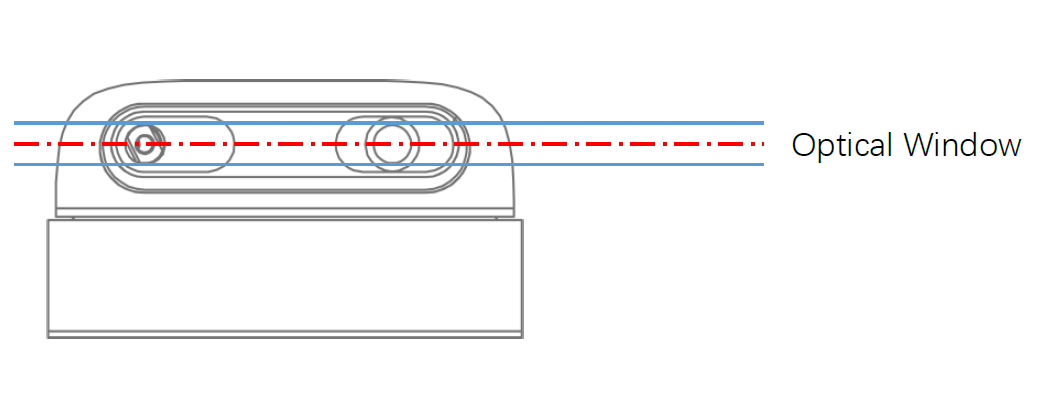
\includegraphics[width=100truemm]{images/rplidar_a2_optical_window.png}
  \label{fig:rplidar_a2_optical_window}
  \caption{RPLiDAR A2 Optical Window}
\end{figure}

\subsection{RPLiDAR A2の座標系}

RPLiDAR A2は少々特殊な座標系を持っており,その向きは図\ref{fig:rplidar_a2_coordinate_system}に示す通りになっています.

\begin{figure}[ht]
  \centering
  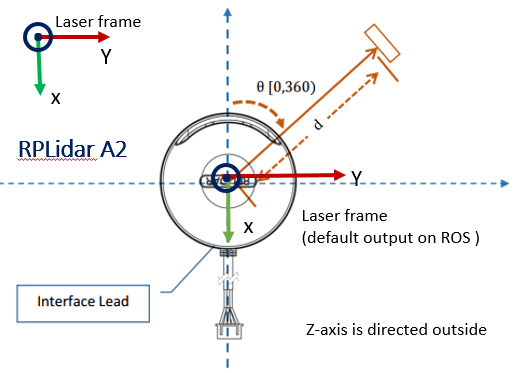
\includegraphics[width=100truemm]{images/rplidar_a2_coordinate_system.png}
  \label{fig:rplidar_a2_coordinate_system}
  \caption{Coordinate System of RPLiDAR A2}
\end{figure}

図を見るとわかるのですが,ROS REP:103で推奨されている座標系と一致していません(Z軸周りに180度回転させた向きになっている).
そのため,モデルの見た目とセンサデータの座標変換とを両立させるために,ジョイントの向きを図\ref{fig:rplidar_a2_coordinate_system}の通りにし,モデルの見た目を180度回転させる,という処理が必要になります.

\subsection{\textsf{lidar.xacro}の記述}

以上を踏まえて,\textsf{lidar.xacro}を記述します.
\textsf{urdf/}ディレクトリ以下に\textsf{lidar/}ディレクトリを作り,その中にコード\ref{code:lidar_xacro}の内容を記述したファイル\textsf{lidar.xacro}を作成します.

\begin{lstlisting}[language=XML, label=code:lidar_xacro, caption=\textsf{lidar.xacro}]
<?xml version="1.0"?>
<robot xmlns:xacro="http://ros.org/wiki/xacro">
  <xacro:macro name="lidar" params="parent *joint_origin">
    <joint name="lidar_joint" type="fixed">
      <xacro:insert_block name="joint_origin"/>
      <parent link="${parent}"/>
      <child link="lidar_link"/>
    </joint>

    <link name="lidar_link">
      <visual>
        <geometry>
          <mesh filename="package://adamr2_description/meshes/lidar_link.STL"/>
        </geometry>
        <material name="blue">
          <color rgba="0.0 0.0 1.0 1.0"/>
        </material>
      </visual>
    </link>
  </xacro:macro>
</robot>
\end{lstlisting}

\end{document}